%"{'classe':('PSI'),'chapitre':'tec_jeq','type':('application'),'titre':'Détermination de l\\'inertie équivalente de réducteurs', 'source':'','comp':[],'corrige':True}"
\setchapterimage{gears}
\chapter*{Application \arabic{cptApplication} \\ 
Détermination de l'inertie équivalente de transmetteurs -- \ifprof Corrigé \else Sujet \fi}
\addcontentsline{toc}{section}{Application \arabic{cptApplication} : Détermination de l'inertie équivalente de transmetteurs -- \ifprof Corrigé \else Sujet \fi}

\iflivret \stepcounter{cptApplication} \else
\ifprof  \stepcounter{cptApplication} \else \fi
\fi

%\setcounter{question}{0}
%\marginnote{Mines Ponts PSI -- 2003.}
%\marginnote[1cm]{
%\UPSTIcompetence[2]{B2-10}
%}
%\begin{marginfigure}
%\centering
%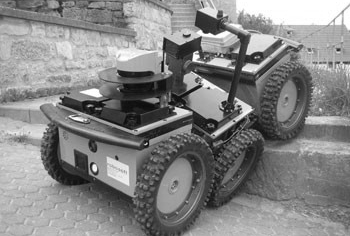
\includegraphics[width=4cm]{fig_00}
%\end{marginfigure}
\newcommand{\repappli}{\repRel/PSI_ExercicesCompetences/TEC/TEC-04-Meq-Jeq/}
\newcommand{\appli}{23_TrainSimple}

\renewcommand{\nomExo}{Cy_05_01_Application_00_Reducteurs}

\renewcommand{\appli}{23_TrainSimple}
\graphicspath{{\repStyle/png}{\repappli\appli/images}}
\input{\repappli\appli/\appli}

%\renewcommand{\appli}{26_RoueMotrice}
%\graphicspath{{\repStyle/png}{\repappli\appli/images}}
%\input{\repappli\appli/\appli}

%\newpage


\renewcommand{\appli}{38_Treuil}
\graphicspath{{\repStyle/png}{\repappli\appli/images}}
\input{\repappli\appli/\appli}

\renewcommand{\appli}{36_VisEcrou}
\graphicspath{{\repStyle/png}{\repappli\appli/images}}
\input{\repappli\appli/\appli}

\renewcommand{\appli}{94_Taurus}
\graphicspath{{\repStyle/png}{\repappli\appli/images}}
\input{\repappli\appli/\appli}

%\newpage


\renewcommand{\appli}{34_ControlX}
\graphicspath{{\repStyle/png}{\repappli\appli/images}}
\input{\repappli\appli/\appli}

\newpage

\renewcommand{\appli}{33_Centrifugeuse}
\graphicspath{{\repStyle/png}{\repappli\appli/images}}
\input{\repappli\appli/\appli}


